\documentclass[a4paper,12pt]{report}
\usepackage[toc,page]{appendix}
\usepackage{amsmath}
\usepackage{float}
\usepackage{graphicx}
\usepackage{subfig}
\usepackage{amssymb}
\usepackage{geometry}
\usepackage{array}
\usepackage{tcolorbox}
\usepackage[normalem]{ulem}

\usepackage{setspace}
 \geometry{
 a4paper,
 total={170mm,257mm},
 left=20mm,
 top=20mm,
 }
\usepackage{tikz}
\usepackage{pgfplots}
\usetikzlibrary{shapes, arrows.meta, decorations.pathreplacing, positioning, petri, fit, calc}
\tikzstyle{startstop} = [circle, minimum size=1cm ,text centered, draw=black]
\tikzstyle{neuron} = [circle, minimum size=1cm ,text centered, draw=red, fill=gray!30]
\tikzstyle{neuronEll} = [ellipse, minimum size=1cm ,text centered, text width=2cm, draw=red, fill=gray!30]
\tikzstyle{process} = [rectangle, minimum width=2cm, minimum height=0.5cm, text centered, text width=3cm, draw=black, fill=blue!30]
\tikzstyle{detail} = [rectangle, minimum width=1.5cm, minimum height=0.5cm, text justified, text width=2.6cm, fill=white!30]
\tikzstyle{smalldetail} = [rectangle, minimum width=2cm, minimum height=1cm, text centered, text width=2cm]
\tikzstyle{largedetail} = [rectangle, minimum width=3cm, minimum height=1cm, text centered, text width=4cm, fill=white!30]
\tikzstyle{box} = [rectangle, minimum width=5cm, minimum height=9cm, text centered, text width=4cm, draw=black, fill=white!30]

\usepackage[utf8]{inputenc}

% Default fixed font does not support bold face
\DeclareFixedFont{\ttb}{T1}{txtt}{bx}{n}{10} % for bold
\DeclareFixedFont{\ttm}{T1}{txtt}{m}{n}{10}  % for normal

% Custom colors
\usepackage{color}
\definecolor{deepblue}{rgb}{0,0,0.5}
\definecolor{deepred}{rgb}{0.6,0,0}
\definecolor{deepgreen}{rgb}{0,0.5,0}

\usepackage{listings}

% Python style for highlighting
\newcommand\pythonstyle{\lstset{
language=Python,
basicstyle=\ttm,
otherkeywords={self},             % Add keywords here
keywordstyle=\ttb\color{deepblue},
emph={MyClass,__init__},          % Custom highlighting
emphstyle=\ttb\color{deepred},    % Custom highlighting style
stringstyle=\color{deepgreen},
frame=tb,                         % Any extra options here
showstringspaces=false            % 
}}


% Python environment
\lstnewenvironment{python}[1][]
{
\pythonstyle
\lstset{#1}
}
{}

% Python for external files
\newcommand\pythonexternal[2][]{{
\pythonstyle
\lstinputlisting[#1]{#2}}}

% Python for inline
\newcommand\pythoninline[1]{{\pythonstyle\lstinline!#1!}}


\begin{document}
\tableofcontents

\title{Support Vector Machines \\ Effective algorithm for non-linear classification \\ (non-linear decision boundary)}
\maketitle
\part{Week 7}
Support Vector Machine is a supervised machine learning algorithm which can be used for both classification or regression challenges. However, it is mostly used in classification problems. Regression cannot deal with complex data. SVM works well on small dataset, but can be stronger and more powerful in building complex models.
\section{Optimization objectives}
\subsection{cost function}
\begin{itemize}
\item For Logistic regression:
\begin{align}
h_{\theta}(x) = \frac{1}{1+e^{-\theta^T x}}
\begin{cases}
    \small{\text{if } y=1 \text{, we would want } h_{\theta}(x) \approx 1 \Rightarrow \theta^T x>>0} \\
		\small{\text{if } y=0 \text{, we would want } h_{\theta}(x) \approx 0 \Rightarrow \theta^T x<<0} \\
  \end{cases}
\end{align}
\end{itemize}
\begin{itemize}
\item In Logistic Regresssion, for each training example, the cost function is :
\end{itemize}
\begin{align}
\begin{split}
cost &= -y \mathrm{Log}(h_{\theta}(x)) - (1-y)\mathrm{Log}(1-h_{\theta}(x)) \\
&= -y \mathrm{Log}\left(\frac{1}{1+e^{-\theta^T x}}\right) - (1-y)\mathrm{Log}\left(1-\frac{1}{1+e^{-\theta^T x}}\right)
\end{split}
\end{align}
\\
\\
\begin{itemize}
\item SVM: to build the SVM, we modify the cost function
\end{itemize}
\begin{table}
\centering
\begin{tabular}{l |l | l}
\hline
& if $y=+1$ &  if $y=0$  \\
& 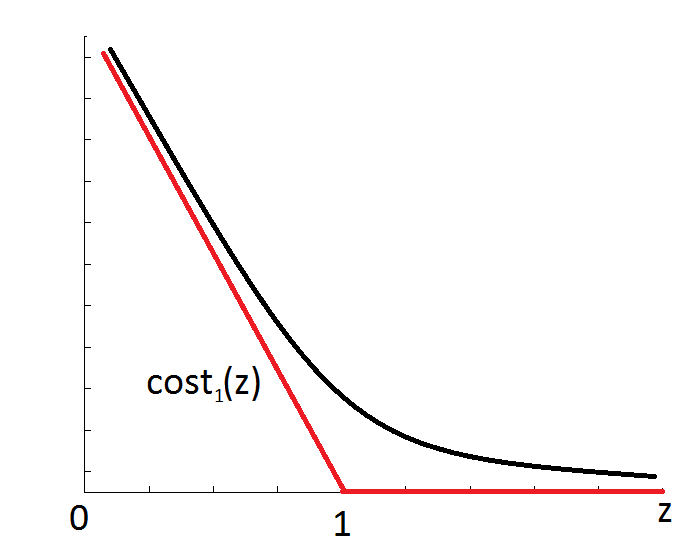
\includegraphics[totalheight=3 cm]{y1.png} & 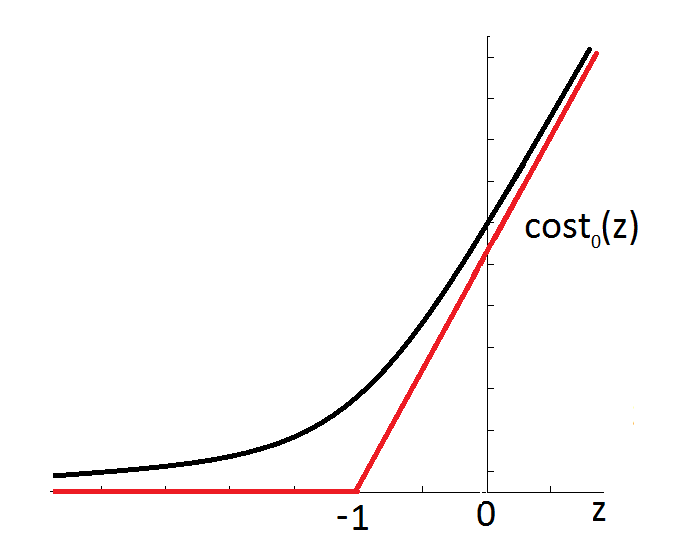
\includegraphics[totalheight=3 cm]{y0.png} \\
new cost function (SVM) & (cost$_1$(z)) [red line] & (cost$_0$(z)) \\
new condition & (want $\theta^T x \geq 1$) & (want $\theta^T x \leq -1$) \\
\hline
\end{tabular}
\end{table}

\begin{align}
cost = cost_1(\theta^T x) + cost_0(\theta^T x)
\end{align}

\subsection{SVM Optimization Objective}
\begin{itemize}
\item For Logistic Regression, the optimization objective is:
\end{itemize}
\begin{align}
min_{\theta} \text{\ } \frac{1}{m} \left[ \sum_{i=1} ^m y^{(i)} \left( -\mathrm{Log} h_{\theta}(x^{(i)}) \right) + (1-y^{(i)}) \left( -\mathrm{Log} (1-h_{\theta}(x^{(i)})) \right) \right]  + \frac{\lambda}{2m} \sum_{j=1} ^n \theta_j ^2
\end{align}

\begin{itemize}
\item For Support Vector Machine, the formulation of the optimization objective is:

\begin{align}
min _{\theta}\text{\ } \frac{1}{m} \left[ \sum_{i=1} ^m y^{(i)} cost_1 (\theta^T x^{(i)}) + (1-y^{(i)}) cost_0( \theta^T x^{(i)})\right] + \frac{\lambda}{2m} \sum_{j=1} ^{n} \theta_j ^2 
\end{align}

SVM uses different conventions than Linear Regression
\begin{itemize}
\item $\frac{1}{m}$ term is eliminated
\item $\lambda$ is replaced by $C$ which now acts on the main term, rather than the regularization term: 
\end{itemize}
\begin{align}
min _{\theta}\text{\ } C \left[ \sum_{i=1} ^m y^{(i)} cost_1 (\theta^T x^{(i)}) + (1-y^{(i)}) cost_0( \theta^T x^{(i)})\right] + \frac{1}{2} \sum_{j=1} ^{n} \theta_j ^2
\end{align}
\end{itemize}
Unlike Linear Regression, SVM does not output a probability but values $\in \{0,1\}$:

\section{SVM - Large Margin Classifier}
\subsection{constraint for SVM}
\begin{itemize}
\item Optimization objective: 
\begin{align}
min _{\theta} \ C \left[ \sum_{i=1} ^m y^{(i)} cost_1 (\theta^T x^{(i)}) + (1-y^{(i)}) cost_0( \theta^T x^{(i)})\right] + \frac{\lambda}{2} \sum_{j=1} ^{n} \theta_j ^2
\end{align}
\begin{figure}[H]
	\centering
        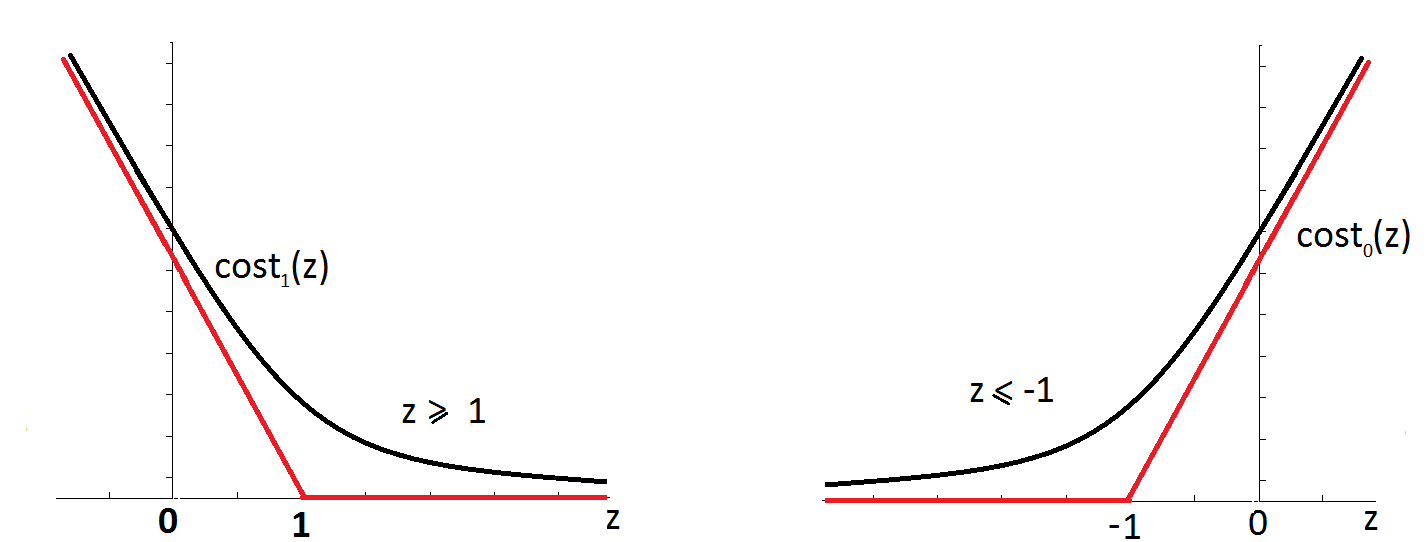
\includegraphics[totalheight=4 cm]{y0-1.png}
\end{figure}
\end{itemize}
\begin{itemize}
\item what does it take to make the cost function small ($min_{\theta} cost = 0$)
\begin{align}
\begin{cases}
    \text{if $y=1$ we want} & cost_1 \theta^T x = 0 \ \Rightarrow  \ \theta^T x \geq 1  \\
    \text{if $y=0$ we want} & cost_0 \theta^T x = 0 \ \Rightarrow  \  \theta^T x \leq -1 \\
  \end{cases}
\end{align}
\end{itemize}
Note that in contrast, for Linear Regression we just needed $\theta^T x \geq 0$ if $y=1$, and $\theta^T x \leq 0$ if $y=0$

\subsection{For large C}
\begin{itemize}
\item SVM Optimization objective
\end{itemize}
\begin{align}
min _{\theta} \ C \left[ \sum_{i=1} ^m y^{(i)} cost_1 (\theta^T x^{(i)}) + (1-y^{(i)}) cost_0( \theta^T x^{(i)})\right] + \frac{1}{2} \sum_{j=1} ^{n} \theta_j ^2 
\end{align}
In order to minimize the cost for large C, we would want:
\begin{align}
\left[ \sum_{i=1} ^m y^{(i)} cost_1 (\theta^T x^{(i)}) + (1-y^{(i)}) cost_0( \theta^T x^{(i)})\right] = 0
\end{align}
so:
\begin{align}
\begin{cases}
    \text{whenever $y=1$ we want} & cost_1 \theta^T x = 0 \ \Rightarrow  \ \theta^T x \geq 1  \\
    \text{whenever $y=0$ we want} & cost_0 \theta^T x = 0 \ \Rightarrow  \  \theta^T x \leq -1 \\
  \end{cases}
\end{align}
so, the optimization problems becomes:
\begin{align}
min_{\theta} C \times 0 + \frac{1}{2} \sum_{i=1} ^{n} \theta_j ^2
\end{align}
with the constraint:
\begin{align}
\begin{cases}
    \theta^T x^{(i)} \geq 1  \text{\ if $y^{(i)}=1$}\\
    \theta^T x^{(i)} \leq -1  \text{\ if $y^{(i)}=0$}\\
  \end{cases}
\end{align}

\subsection{Visualization of the decision boundary for large C}
In this linearly separable case, the 2 dashed lines are possible boundary decisions. However, SVM would choose the decision boundary resulting in the largest margin possible. Hence, SVM is also called 'Large Margin Classifier'.
\begin{figure}[H]
	\centering
        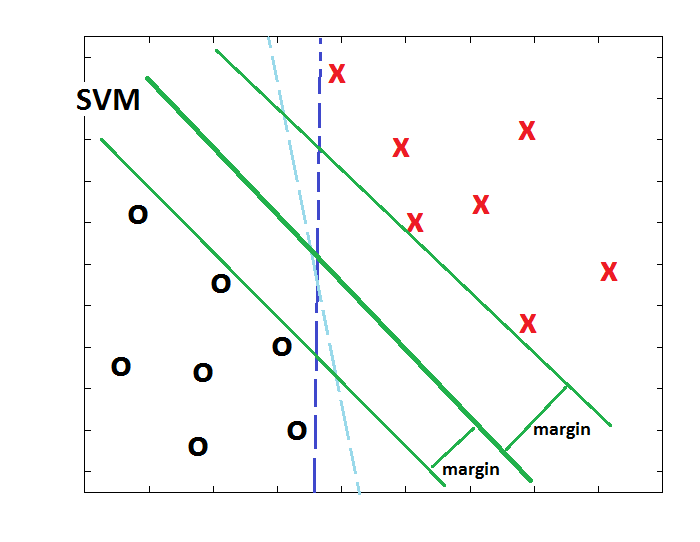
\includegraphics[totalheight=4 cm]{SVM_margin.png}\caption{linearly separable data}
\end{figure}
\begin{itemize}
\item Large Margin Classifier in presence of outliers (very large C)
\end{itemize}

\begin{figure}[H]
	\centering
        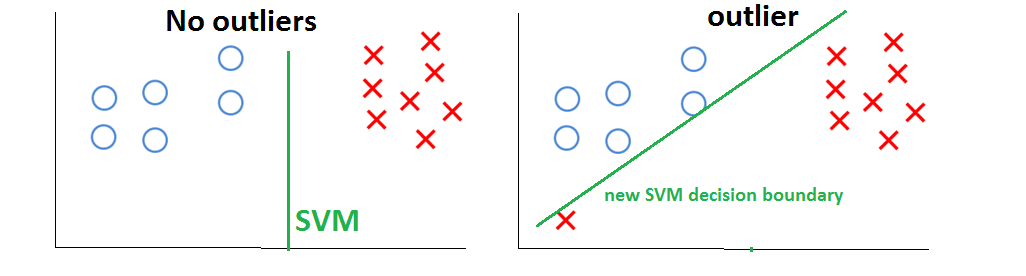
\includegraphics[totalheight=4 cm]{outlier.png}\caption{if C is large, SVM will take into accoutn the presence of the outlier. Bit if C is not too large, there is less overfitting. }
\end{figure}

\section{Mathematics behind Large Margin classifier}
\begin{itemize}
\item Optimization Objective for SVM (large C)
\end{itemize}

\begin{align}
min_{\theta} = \frac{1}{2} \sum_{j=1} ^n \theta_j ^2 \text{ \ with}
\begin{cases}
    \theta^T x^{(i)} \geq 1  \text{\ if $y^{(i)}=1$}\\
    \theta^T x^{(i)} \leq -1  \text{\ if $y^{(i)}=0$}\\
  \end{cases}
\end{align}

\begin{itemize}
\item Assumptions: 
\begin{itemize}
\item $\theta_0 = 0$ 
\item only 2 features ($n$=2)
\end{itemize}
\end{itemize}

\begin{figure}[H]
	\centering
        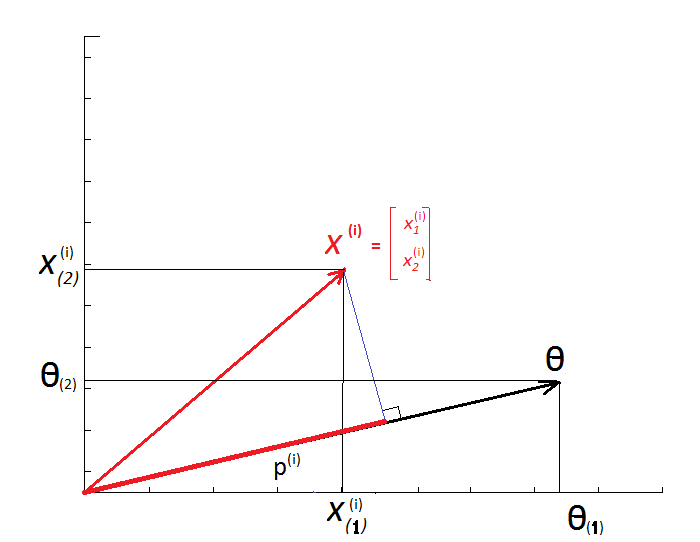
\includegraphics[totalheight=4 cm]{vectorsxtheta.png}\caption{}
\end{figure}

\begin{itemize}
\item Optimization objective:
\end{itemize}
\begin{align}
min_{\theta} \frac{1}{2} (\theta_1 ^2 + \theta_2 ^2) = \frac{1}{2} (\sqrt{\theta_1 ^2 + \theta_2 ^2}^2) = \frac{1}{2} ||\theta||^2
\end{align}
where $\theta= \left[ \begin{smallmatrix} \theta_1 & \theta_2 \end{smallmatrix} \right]$

\begin{itemize}
\item Vector Inner Product $\theta^T x^{(i)} = ?$
\end{itemize}

\begin{align}
\theta^T x^{(i)} = p^{(i)} ||\theta|| = \theta_1 x^{(i)}_1 + \theta_2 x^{(i)} _2
\end{align}
So the \textbf{constraint} $\theta ^T x^{(i)} \geq 1$ becomes :
\begin{align}
p^{(i)} ||\theta|| \geq 1
\end{align}

\begin{itemize}
\item SVM Decision Boundary: What SVM is more likely to choose for the decision boundary
\begin{itemize}
\item case 1:
\begin{figure}[H]
	\centering
        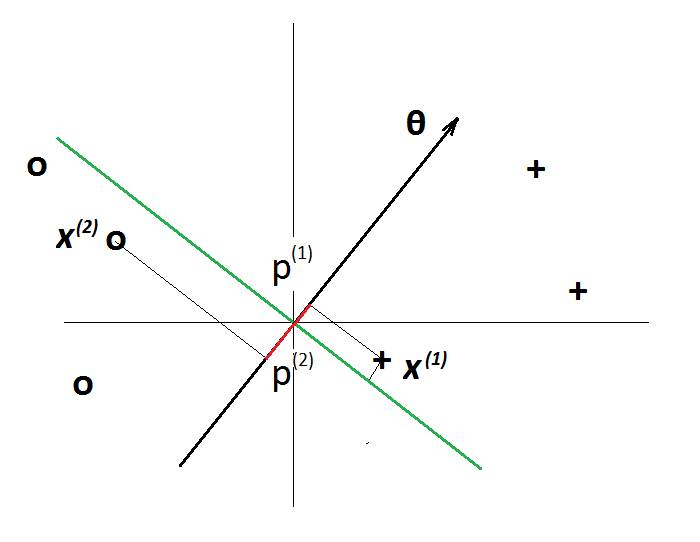
\includegraphics[totalheight=4 cm]{case1decboundary.png}\caption{}
\end{figure}
The projection of $x^{(1)}$ and $x^{(2)}$ on $\theta$ axis gives: $p^{(1)}$ and $p^{(2)}$. Those 2 length are small. So to satisfy the constraint $p^{(1)} ||\theta|| \geq 1$ ($y$=1), we would need $||\theta||$ to be large. Similarly, to satisfy the constraint $p^{(2)} ||\theta|| \leq 1$ ($y$=-1), we would need $||\theta||$ to be large also. However this goes opposite to the optimization objective $min_{\theta} ||\theta||^2$ which requires $||\theta||$ to be small. So this decision boundary is not a good start. \\
\item case 2:
\begin{figure}[H]
	\centering
        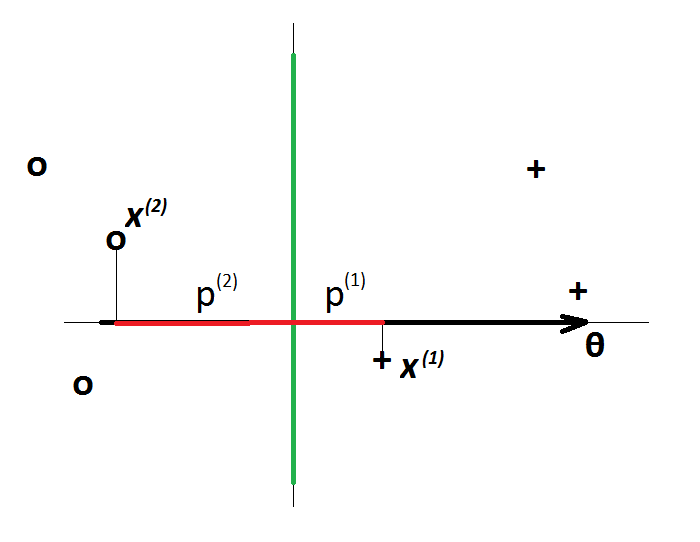
\includegraphics[totalheight=4 cm]{case2decboundary.png}\caption{}
\end{figure}
In this case, $p^{(1)}$ and $p^{(2)}$ are large. So, the constraint $p^{(1)} ||\theta|| \geq 1$ requires $||\theta||$ to be small, which does go against along a minimization of $||\theta||^2$ for the optimization objective.
\end{itemize}
\end{itemize}
\textbf{SVM is trying to maximize} $p^{(i)}$.
\\
Note that with the restriction $\theta_0 = 0$, it just means that the decision boundary must pass through 0.



\section{SVM Kernels I}
The Kernels enable to develop complex non linear classifier.
\subsection{Example}
For non-linear decision boundary, a first approach coudl be the use of polynomial features : $\theta^T x = \theta_0 + \theta_1 x_1 + \theta_2 x_2 + \theta_3 x_1 x_2 + \theta_4 x_1 ^2 ... $, where $\theta^T x \geq 1 $ predicts $y=1$.
\begin{figure}[H]
	\centering
        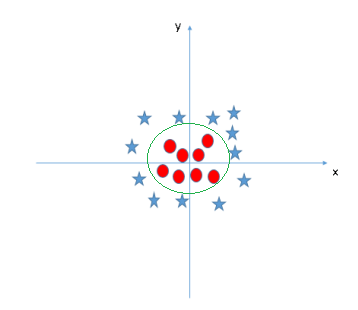
\includegraphics[totalheight=4 cm]{SVM_8.png}\caption{}
\end{figure}
This can also be written:
\begin{align}
\theta_0 + \theta_1 f_1 + \theta_2 f_2 + \theta_3 f_3 + \theta_4 f_4 ...
\end{align}
where $f_1=x_1$, $f_2 = x_2$, $f_3=x_1 x_2$, etc...\\
\textbf{But, is there a better set of features?}\\

\subsection{landmarks}
Given $x$, compute new feature depending on proximity to landmarks $l^{(1)}$, $l^{(2)}$ and $l^{(3)}$.
\begin{figure}[H]
	\centering
        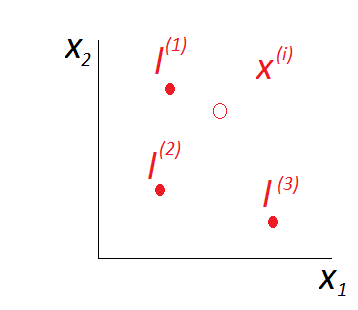
\includegraphics[totalheight=4 cm]{landmarks.png}\caption{}
\end{figure}
\begin{align}
\begin{split}
f_1 &= \text{measure of similarity of \ } (x,l^{(1)}) = exp\left(-\frac{||x-l^{(1)}||^2}{2 \sigma^2} \right) \\
f_2 &= \text{measure of similarity of \ } (x,l^{(2)}) = exp\left(-\frac{||x-l^{(2)}||^2}{2 \sigma^2} \right) \\
f_3 &= \text{measure of similarity of\ } (x,l^{(3)}) = exp\left(-\frac{||x-l^{(3)}||^2}{2 \sigma^2} \right)
\end{split}
\end{align}
$exp\left(-\frac{||x-l||^2}{2 \sigma^2} \right)$ is called the Kernel function (similarity function), and in this particular instance, we have a Gaussian Kernel. The Kernel between $x$ and $l$ is also noted $K(x,l)$
\begin{align}
f_1 = exp\left(-\frac{||x-l^{(1)}||^2}{2 \sigma^2} \right) = exp\left(-\frac{\sum _j=1 n (x_j - l_j^{(1)})^2}{2 \sigma^2} \right) 
\end{align}
If $x \approx l^(1)$ ($x$ is close to $l^{(1)}$ $\Rightarrow$ $f_1 \approx exp(0) \approx 1$ \\
If $x$ is far from $l^{(1)}$ $\Rightarrow$ $f_1 \approx exp(-(large Nbr)/2 \sigma^2) \approx 0$

\begin{itemize}
\item Example:
\begin{itemize}
\item Hypothesis: Predict 1 when $\theta_0 + \theta_1 f_1 + \theta_2 f_2 + \theta_3 f_3 \geq 0$ \\
Let's say the minimization gives: $\theta_0 = -0.5$, $\theta_1 = 1$, $\theta_2 = 1$, $\theta_3 = 0$
\end{itemize}
\end{itemize}
\begin{figure}[H]
	\centering
        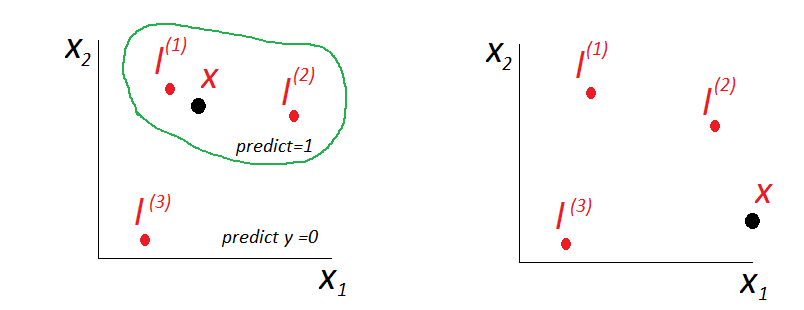
\includegraphics[totalheight=4 cm]{landmarksExple.png}\caption{}
\end{figure}
\begin{itemize}
\item Let's consider a training example $x$. Because $x$ is close to $l^{1}$ and far from $l^{(2)}$ and $l^{(3)}$, $f_1 \approx 1$, $f_2 \approx 0$ and $f_3 \approx 0$. 
\begin{align}
\theta_0 + \theta_1 \times 1 + \theta_2 \times 0 + \theta_3 \times 0 = 0.5 \geq 0 \Rightarrow \text{we predict\ } y=1
\end{align}
\end{itemize}
\begin{itemize}
\item Let's consider another training example $x^{(2)}$. Because $x^{(2)}$ is far from all landmarks $f_1 \approx 0$, $f_2 \approx 0$ and $f_3 \approx 0$. 
\begin{align}
\theta_0 + \theta_1 \times 0 + \theta_2 \times 0 + \theta_3 \times 0 = -0.5 \leq 0 \Rightarrow \text{we predict\ }  y=0
\end{align}
\end{itemize}
We can also notice that for points close to $l^{(1)}$ and $l^{(2)}$, we end up predicting positive, and for points far away, we end up predicting negative. So the decision boundary would be as shown by the green line.


\subsection{How to choose the landmarks}
In practice the landmarks will be at exactly the same position as the training examples.
\begin{itemize}
\item Given a set of training examples $(x^{(1)}, y^{(1)}), (x^{(2)}, y^{(2)}), (x^{(3)}, y^{(3)}), ...(x^{(m)}, y^{(m)}) $
\item Choose $l^{(1)}=x^{(1)}$, $l^{(2)}=x^{(2)}$, ....., $l^{(m)}=x^{(m)}$
\item Given an example $x^{(i)} \in \mathbb{R}^{n+1}$ (or $\in \mathbb{R}^n$):\\
 $l^{(1)}=x^{(1)}$, $l^{(2)}=x^{(2)}$, ....., $l^{(m)}=x^{(m)}$
\begin{align}
\begin{split}
f_1 &= \text{similarity} (x^{(i)}, l^{(1)})\\
f_2 &= \text{similarity} (x^{(i)}, l^{(2)})\\
. & ...\\
f_i & \text{similarity} (x^{(i)}, l^{(i)}) = 1 \\
. & ...\\
f_m &= \text{similarity} (x^{(i)}, l^{(m)})
\end{split}
\end{align}
So the new feature vector $f^{(i)}=\left[ \begin{smallmatrix} f_0 \\ f_1 \\..\\..\\.. f_m \end{smallmatrix}\right]$ with $f_0 =1$. \\
\item To get $\theta$, we use the SVM minimization algorithm:
\begin{align}
min_{\theta} C \sum_i=1 ^{m} \left[ y^{(i)} cost_1(\theta^T f^{(i)} + (1-y^{(i)}) cost_0(\theta^T f^{(i)} \right] + \frac{1}{2}\sum_{j=1} ^m \theta_j^2
\end{align}
Note that most SVM packages replace $\theta^2 = \theta^T \theta$ by $\theta^T M \theta$, where $M$ is a matrix that depends on the Kernel used.
\end{itemize}

\subsection{How to choose C and $\sigma$}
\begin{itemize}
\item How to choose C($=1/\lambda$):
\begin{itemize}
\item Large C: lower bias, high variance
\item small C: large bias, low variance
\end{itemize}
\end{itemize}


\begin{itemize}
\item How to choose $\sigma^2$:
\begin{itemize}
\item Large $\sigma^2$: features $f_i$ vary more smoothly $\Rightarrow$ higher bias and lower variance
\item small $\sigma^2$: features $f_i$ vary less smoothly $\Rightarrow$ higher variance and lower bias
\end{itemize}
\end{itemize}

\section{How to use an SVM}
\begin{itemize}
	\item use SVM packages ('liblinear', 'libsvm'...) to solve for parameters $\theta$
	\item Need to specify:
	\begin{itemize}
		\item Choice of parameter C
		\item Choice of kernel (similarity function)
			\begin{itemize}
				\item when $n$ large and $m$ small: No kernel ("linear" kernel) (=standard linear classifier)
				\item when $n$ small and $m$ large: use Gaussian Kernel -- need to choose $\sigma^2$ \\
					Note: do perform feature scaling before using the Gaussian Kernel.\\
Not all similarity functions are valid kernels. They must satisfy "Mercer's Theorem," which guarantees that the SVM package's optimizations run correctly and do not diverge.
You want to train C and $\sigma$ using the training and cross-validation datasets.
\end{itemize}
\end{itemize}
\end{itemize}
\section{Multi-class Classification}
\begin{itemize}
\item Many SVM libraries have multi-class classification already built-in. \\
	\item You can use the one-vs-all method
\end{itemize}
\begin{itemize}
	\item Logistic Regression vs. SVMs
		\begin{itemize}
			\item if $n$ large (relative to $m$) $\Rightarrow$ use logistic regression, or linear Kernel
			\item if $n$ small and $m$ is intermediate $\Rightarrow$ use SVM with a Gaussian Kernel
			\item if $n$ small and $m$ large, $\Rightarrow$ manually create/add more features, $\Rightarrow$ use logistic regression or SVM without a kernel.
Note: a neural network is likely to work well for any of these situations, but may be slower to train.
		\end{itemize}
\end{itemize}

\begin{appendices}
\section{question}
Consider the training set, where 'x' denotes positive examples ($y=1$) and 'o' denotes negative examples ($y=0$). Suppose you train an SVM (which will predict 1 when $\theta_0 + \theta_1 x_1 + \theta_2 x_2 \geq 0)$. What values might the SVM give for $\theta_0$, $\theta_1$ and $\theta_2$?
\begin{figure}[H]
	\centering
        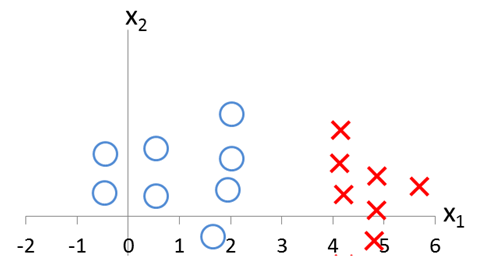
\includegraphics[totalheight=4 cm]{question.png}\caption{}
\end{figure}

Response: $\theta_-3$, $\theta_1=1$ and $\theta_2=0$

\section{Vector inner product ($u^T v$)}

\begin{figure}[H]
	\centering
        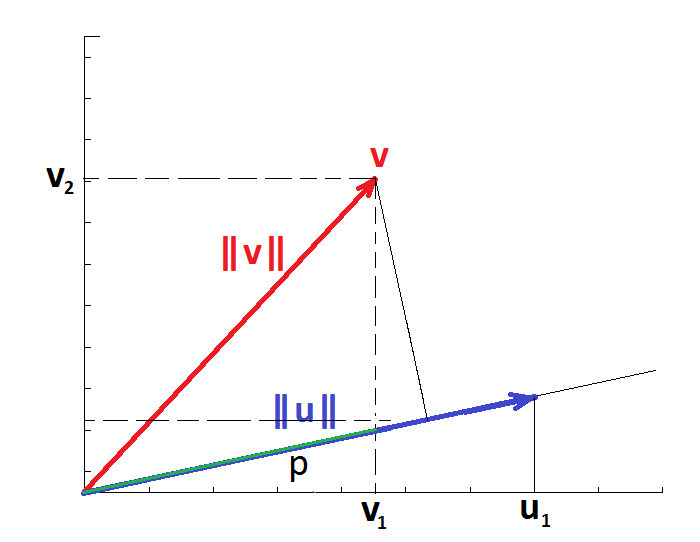
\includegraphics[totalheight=4 cm]{vectors.png}\caption{$p$ is the length of projection of $v$ on $u$ (where $p$ is $\pm$-ive)} 
\end{figure}
Let's consider 2 vectors $u=\begin{smallmatrix} u_1 \\ u_2 \end{smallmatrix}$ and $v=\begin{smallmatrix} v_1 \\ v_2 \end{smallmatrix}$. \\
$||u|| = \sqrt{u_1 ^2 + u_2 ^2} \in \mathbb{R}$.

\begin{itemize}
\item $p$ is the length of the projection of $v$ on $u$, where $p \in \mathbb{R}$ and can be positive or negative \\
\begin{align}
u^T v = p . ||u|| = u_1 v_1 + u_2 v_2
\end{align}
\end{itemize}

\section{SVM Intro}
In this algorithm, we plot each data item as a point in $n$ dimensional space (where $n$ is the number of features), with the value of each feature being the value of a particular coordinate. Then we perform classification by finding the hyper-plane that differentiate the 2 classes. Support Vector Machine is a frontier which best segregates the 2 classes (hyper plane line).
\begin{figure}[H]
	\centering
        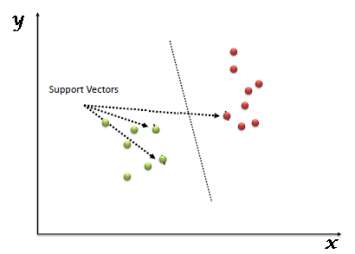
\includegraphics[totalheight=4 cm]{SVM_1.png}\caption{Support vectors are simply the coordinates of individual observation ($x$, $y$).}
\end{figure}

Let's look at a few examples:
\begin{itemize}
\item Scenario 1 \\
Thumb-rule to identify the right hyper-plane: "select the hyper-plane which segregates the 2 classes better". In this scenario, B is the best frontier.
\begin{figure}[H]
	\centering
        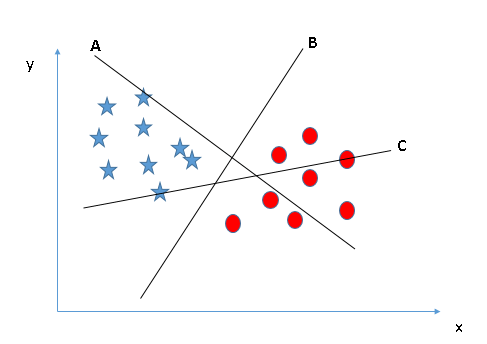
\includegraphics[totalheight=4 cm]{SVM_21.png}
\end{figure}
\end{itemize}

\begin{itemize}
\item Scenario 2 \\
Maximizing the distances between nearest data point (either class) and hyper-plane will help us to decide the right hyper-plane. This distance is called a margin and C has the largest margin. 
\begin{figure}[H]
	\centering
        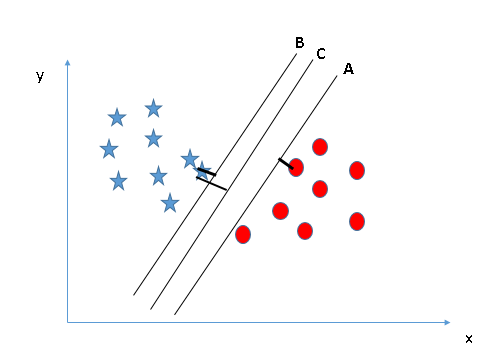
\includegraphics[totalheight=4 cm]{SVM_4.png}
\end{figure}
\end{itemize}

\begin{itemize}
\item Scenario 3 \\
SVM selects the hyper-plane which classifies the classes accurately prior to maximizing the margin. Therefore, the right hyper-plane is A.
\begin{figure}[H]
	\centering
        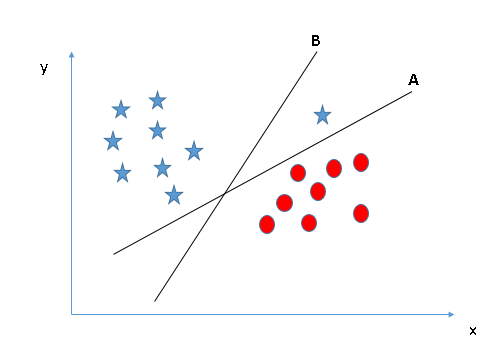
\includegraphics[totalheight=4 cm]{SVM_5.png}
\end{figure}
\end{itemize}

\begin{itemize}
\item Scenario 4 \\
One star at other end is like an outlier for star class. SVM has a feature to ignore outliers and find the hyper-plane that has maximum margin. Hence, SVM is robust to outliers.
\begin{figure}[H]
	\centering
        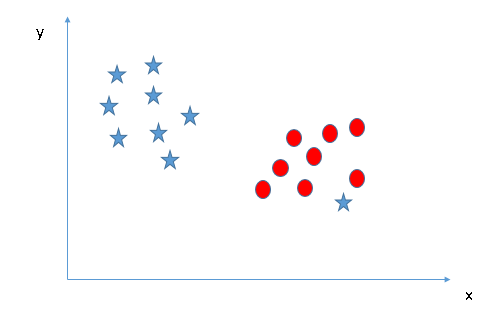
\includegraphics[totalheight=4 cm]{SVM_61.png}
\end{figure}
\end{itemize}

\begin{itemize}
\item Scenario 5 \\
A linear hyperplane between the 2 classes cannot be found. In such a case, we need to map  those vectors to a higher dimension plane so that they get segregated from each other. Here we will add a new features: $z = x^2 + y^2 $ and plot $x$ versus $z$.

\begin{tabular}{ll}
%\hline
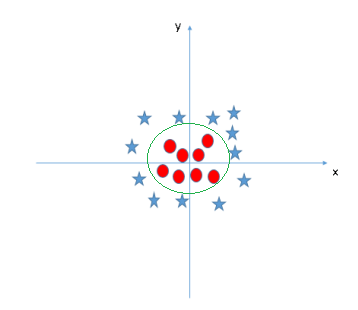
\includegraphics[totalheight=3 cm]{SVM_8.png} & 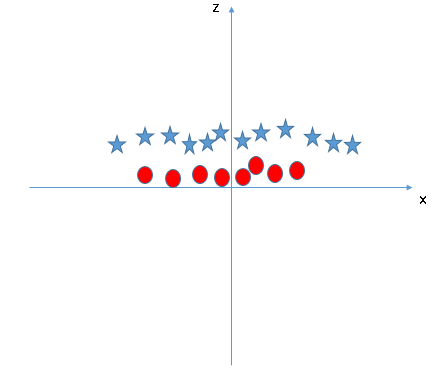
\includegraphics[totalheight=3 cm]{SVM_9.png} \\
%\hline
\end{tabular}
\\
Note that, all values of $z > 0$. \\
SVM has a technique called the Kernel trick. These are functions which takes takes  low dimensional input space and transform it to a higher dimensional space.
When we took at the hyper-plane in original input space, it looks like a circle
\begin{figure}[H]
	\centering
        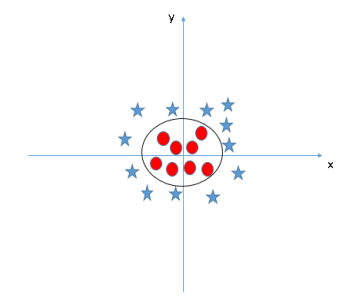
\includegraphics[totalheight=4 cm]{SVM_10.png}
\end{figure} 
\end{itemize}

\end{appendices}

\end{document}